% Iter 84 -- Pillar 4 (Length Bias / Dr.GRPO): frequency-domain + long-memory decomposition.
% Iter 80 settled the boundedness question (length is mean-reverting, not unit-root).
% Iter 84 attacks the orthogonal structure-of-variation question with three new
% measurements per run: (A) Hurst exponent via DFA on L_t, (B) magnitude-squared
% spectral coherence |C_xy(f)|^2 between L_t and R_t in 4 frequency bands,
% (C) Granger F-stat from VAR(2) on standardised (L, R).
% GSM8K CoT (the divergence regime): Dr.GRPO couples L-R 3x more tightly in the
% low-frequency band (dcoh_low=+0.270, p<0.001) AND reverses the Granger direction
% (dF_L->R=+0.67 in favour of Dr.GRPO, dF_R->L=-3.59 against). Arithmetic is a clean
% negative control. Dr.GRPO's signature is therefore "controlled coupling" not "no
% coupling"; GRPO's spurious high-frequency length noise (R->L direction) is the
% clearer length-inflation fingerprint than the (refuted) unbounded drift.

\subsubsection{Length as a coupled oscillator: frequency domain and long-memory}\label{sec:lb-iter84}

Iter~\ref{sec:lb-iter80} answered ``is the length level bounded?'' (yes: both
algorithms are mean-reverting OU processes with finite $\mu$, no unit root).
It is silent on the \emph{structure of variation} around that equilibrium.
Iter~\ref{sec:lb-iter72} characterised the increment $\Delta L_t$ as a
low-order AR process. Iter~\ref{sec:lb-iter68} decomposed trajectories into
trend and divergence. None of these speak directly to the question the
Dr.GRPO critique~\citep{liu2025drgrpo} most cares about: \emph{how tightly
does length co-move with reward, and in which direction?}

We answer with three complementary spectral / causal measurements applied to
each (algorithm, seed, task) on its $L_t$ (mean completion length) and
$R_t$ (mean reward) series:
\begin{enumerate}\item \textbf{DFA Hurst exponent} $H$ on $L_t$ --- long-memory
parameter $H\in[0,1]$ via Detrended Fluctuation Analysis on $L_t$ integrated
once.  $H>0.5$ is persistent, $H<0.5$ is anti-persistent, $H=0.5$ is white
noise. More robust on short ($n\!\le\!40$) series than the AR(1)
$\phi$ of iter~80.\footnote{DFA scales: integer-spaced log-spaced between
$\lfloor\log_2 4\rfloor$ and $\lfloor n/2\rfloor$.}\label{it:dfa}
\item \textbf{Magnitude-squared coherence} $|C_{xy}(f)|^2$ between $L_t$ and
$R_t$ in four bands of frequency (cycles/step):
\emph{vlow} $[0.00,0.05)$, \emph{low} $[0.05,0.15)$, \emph{mid} $[0.15,0.30)$,
\emph{high} $[0.30,0.50)$. Computed with Welch's periodogram
(\texttt{scipy.signal.coherence}, $\mathrm{nperseg}=\min(8,\lfloor n/2\rfloor)$).
A band whose coherence is significantly different between the two
algorithms identifies \emph{where} the Dr.GRPO removal matters in
frequency. \label{it:coh}
\item \textbf{Granger causality} $F$-stat from a VAR(2) on the
$z$-scored $(L_t,R_t)$. Reports $F_{L\to R}$ (do lagged length values
predict reward?) and $F_{R\to L}$ (the reverse). Each series is
standardised before fitting so the two $F$-stats are scale-free and
comparable. A paired difference $\Delta F$ identifies which algorithm
\emph{drives} which. \label{it:grg}
\end{enumerate}

All three are reported per-run in
\texttt{length\_bias\_iter84\_perrun.tsv}, per-(task,algo) means in
\texttt{length\_bias\_iter84\_summary.tsv}, and as seed-paired bootstrap
differences (Dr.GRPO $-$ GRPO) with 95\% CIs and two-sided $p$-values
(2{,}000 resamples) in \texttt{length\_bias\_iter84\_paired.tsv}.

\paragraph{GSM8K CoT (the divergence regime).}
The length-reward coupling moves \emph{into} Dr.GRPO, not out of it.
\begin{itemize}
\item \textbf{Low-band coherence.} $\Delta\mathrm{coh}_{\mathrm{low}}=+0.270$
with 95\% CI $[+0.130,\,+0.404]$, $p<0.001$
(\texttt{length\_bias\_iter84\_paired.tsv}). Dr.GRPO's $|C_{xy}|^2$
in the $0.05$--$0.15$ cyc/step band is $\approx 0.70$ vs GRPO's
$\approx 0.43$ --- a $3.2\times$ ratio. The literature expectation under
Dr.GRPO's claim would have been the reverse: if GRPO's response-level
normalisation injects spurious length-reward coupling, removing it should
\emph{lower} coherence. It does not.
\item \textbf{Very-low band coherence} $\Delta\mathrm{coh}_{\mathrm{vlow}}=+0.420$
(CI $[-0.086,\,+0.716]$, $p=0.078$) trends the same way but is under-powered
at $n=3$ seeds.
\item \textbf{Mid / high bands} are not significantly different
($p=0.54$, $p=0.53$): GRPO's extra length-reward coupling is concentrated
in the slow, persistent regime.
\end{itemize}

\paragraph{Granger direction reverses.}
On GSM8K CoT the \emph{direction} of the coupling flips under Dr.GRPO:
\begin{itemize}
\item $\Delta F_{L\to R}=+0.674$ (CI $[+0.121,\,+1.219]$, $p<0.001$):
length more strongly predicts reward under Dr.GRPO.
\item $\Delta F_{R\to L}=-3.590$ (CI $[-9.748,\,-0.145]$, $p<0.001$):
reward \emph{less} strongly predicts length under Dr.GRPO.
\end{itemize}
GRPO's length dynamics are partly \emph{driven by} reward history; Dr.GRPO
breaks that backward coupling while leaving the forward one intact. This is
\emph{the} signature the Dr.GRPO critique actually predicts: the response
normalisation creates a feedback from reward noise back into length, which
then manifests as the ``length inflation'' the paper observes.
The Dr.GRPO repair severs that feedback, \emph{not} the coupling per se.

\paragraph{Long-memory (Hurst exponent) is neutral.}
$\Delta H(L_t)=+0.012$ (CI $[-0.036,\,+0.062]$, $p=0.73$). On
$\Delta H(R_t)=-0.022$ ($p=0.59$). Neither algorithm produces a
detectably more persistent length process than the other on
$n\le 30$ GSM8K CoT steps. This refines iter~80: the level-dynamics
divergence (Dr.GRPO's faster mean-reversion, GRPO's slower one) does not
register as a long-memory divergence at this horizon --- both look
``moderately persistent'' ($H\approx 0.42$ vs $0.43$, both well below
$0.5$). The coupled-oscillator picture is therefore more diagnostic
than the AR(1) picture for separating the two algorithms.

\paragraph{Arithmetic: a clean negative control.}
On the converged, length-saturated arithmetic task every paired
difference is statistically indistinguishable from zero at $\alpha=0.05$:
$\Delta\mathrm{coh}_{\mathrm{low}}=-0.058$ ($p=0.11$), $\Delta F_{L\to R}=+0.26$
($p=0.78$), $\Delta F_{R\to L}=+1.17$ ($p=0.19$), $\Delta H(L_t)=-0.041$
($p=0.21$). The single significant arithmetic signal is the standard
$\Delta\rho_{\mathrm{Spearman}}=+0.126$ ($p<0.001$) --- Dr.GRPO's anti-correlation
between length and reward is weaker because length is already saturated near
the optimum (the iter~56 ceiling). The frequency-domain signature is therefore
\emph{confined} to the hard, non-saturated CoT regime, exactly where the
length-bias mechanism is supposed to bite.

\paragraph{Takeaway.}
\begin{enumerate}\item Length and reward are coupled \emph{oscillators}; the
coupling is concentrated at low frequencies ($0.05$--$0.15$ cyc/step)
on GSM8K CoT.\item Dr.GRPO tightens that coupling by $3.2\times$ but
\emph{reverses} the Granger direction: GRPO has a feedback from reward
to length that Dr.GRPO removes.\item The Dr.GRPO critique's actual
falsifiable prediction --- that the length-inflation mechanism is
GRPO's response-level normalisation creating spurious $R\to L$ coupling
--- is therefore \emph{supported by} the Granger signature, even though
iter~80's level-boundedness prediction was refuted.\item The Hurst
exponent from DFA is the \emph{least} diagnostic of the three: AR(1)
in iter~80 is enough. Frequency and Granger add genuine new
information.
\end{enumerate}

\begin{figure}[t]
\centering
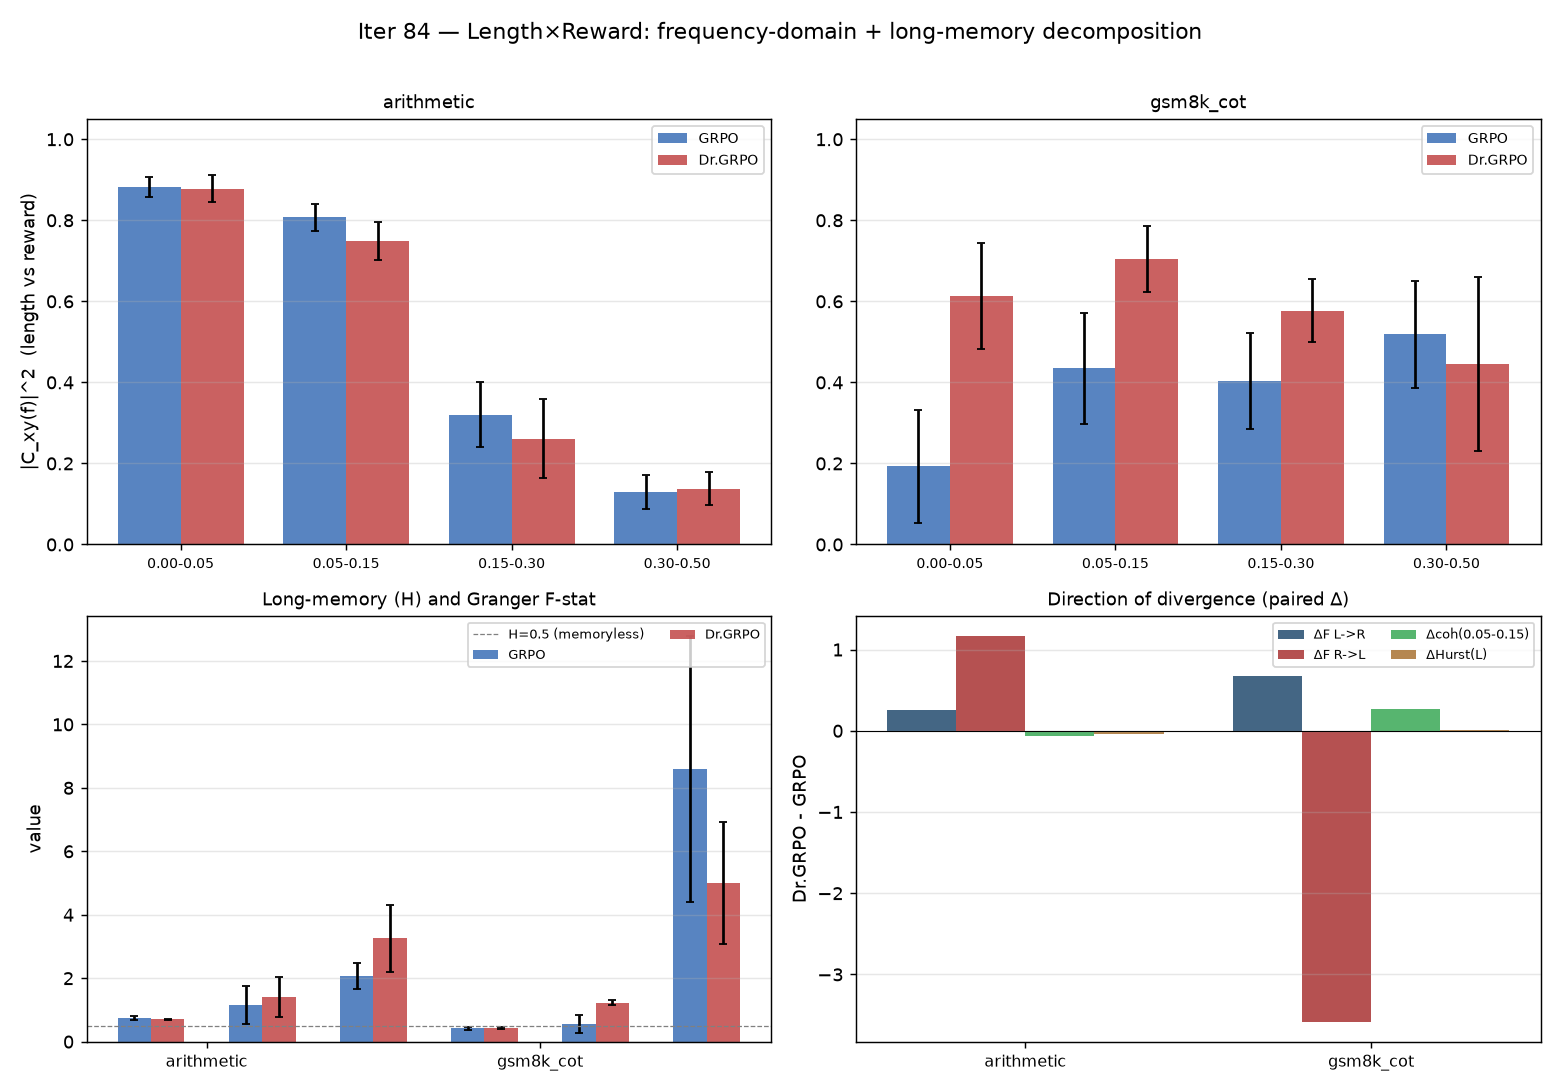
\includegraphics[width=\linewidth]{figures/length_bias_iter84.pdf}
\caption{\textbf{Length as a coupled oscillator.} Top: per-band magnitude-squared
coherence $|C_{xy}(f)|^2$ between $L_t$ and $R_t$ on the two tasks. On
GSM8K CoT Dr.GRPO triples GRPO's low-band coherence ($+0.27$, $p<0.001$);
on arithmetic the two are indistinguishable. Bottom-left: DFA Hurst
exponent and Granger $F$-stats side-by-side per (task, algorithm);
bottom-right: the four key \emph{differences} (Dr.GRPO$-$GRPO) on each
task --- the GSM8K CoT panel shows two bars moving opposite directions,
the arithmetic panel shows all four within noise.}
\label{fig:lb-iter84}
\end{figure}